\documentclass[11pt]{article}

% ---------------------------------------------------------------
% Neutral preprint style (no venue branding).
% Compiles with pdflatex; falls back cleanly if a package is missing.
% Style reference: o1state.tex (same document class, macros, citation style).
% This is a self-contained systems paper, companion to o1state.tex.
% ---------------------------------------------------------------
\usepackage[utf8]{inputenc}
\usepackage[T1]{fontenc}
\usepackage[margin=1in]{geometry}
\usepackage{amsmath,amssymb,amsthm}
\usepackage{graphicx}
\usepackage{booktabs}
\usepackage{array}
\usepackage{siunitx}
\usepackage{microtype}
\usepackage{caption}
\usepackage{subcaption}
\usepackage[dvipsnames]{xcolor}
\usepackage[colorlinks=true,linkcolor=NavyBlue,citecolor=NavyBlue,urlcolor=NavyBlue]{hyperref}
\usepackage{orcidlink}

\graphicspath{{figures/}{../plots/}}

\newtheorem{theorem}{Theorem}
\newtheorem{proposition}{Proposition}
\newtheorem{corollary}{Corollary}
\theoremstyle{definition}
\newtheorem{definition}{Definition}

\newcommand{\R}{\mathbb{R}}
\newcommand{\code}[1]{\texttt{#1}}
% Give the line-breaker slack so long, unbreakable \texttt{} JSON paths in
% running text stretch the line rather than overrun the margin.
\emergencystretch=3em

\title{\bfseries The Organism as a Deployable Asset:\\
Determinism, Provenance, and the Two-Regime Replication Law\\
for Constant-Memory Streaming Learners}

\author{David Tom Foss\,\orcidlink{0009-0004-0289-7154}\\[3pt]
{\normalsize\href{mailto:d.foss@ieee.org}{\texttt{d.foss@ieee.org}}}}
\date{Draft v0.1, August 6, 2026}

\begin{document}
\maketitle

\begin{quote}
\raggedright
\itshape
Every number in this paper is committed in the public repository
\code{github.com/DT-Foss/o1-state} with its generating script and raw JSON.
This is the systems companion to \emph{The O(1)-State Organism} (the
learning-primitives paper); where that paper measures what the organism
learns, this one measures what it is to operate --- reproduce, move,
replicate, and account for.
\end{quote}

\begin{abstract}
A deployed sequence model is not only a function; it is an operational
object that must reproduce, move between machines, replicate across a fleet,
and answer for what it knows. We factor the deployment problem the way the
system is built: intelligence stays small and constant, knowledge lives
outside the weights in frozen, hashed files, and the properties that decide
deployability are therefore \emph{systems} properties, not language-quality
properties. We measure four of them on a constant-memory streaming learner
whose entire living state is a small, portable, forkable artifact.
\textbf{(i) Determinism at production scale.} A \num{50000384}-token run
($d{=}512$) rerun 11 days later, in a different operating-system process,
through a mid-stream reconnect, reproduces all \num{97657} chunk records
bit-identically on every deterministic field --- chunk index, gate decision,
all three surprise streams, and threshold: the per-chunk deterministic-field
maximum difference over the entire run is exactly \num{0.0}. The only field
that moves is wall-clock time. Same-seed variance on the recorded calculus is
zero; the second seed lands at a gate rate of \num{0.1986} against
\num{0.1984}. \textbf{(ii) Provenance as a system property.} Frozen,
SHA-256-hashed knowledge files replay bit-exactly from stream coordinates ---
in text (5/5), in a pixel world \emph{through} a world mutation (5/5), and
through a third-party 3D game engine we did not write (5/5 across episodes) ---
and the file transfers: a fresh reader dosed with the file beats its no-file
twin by \num{0.056} negative log-likelihood on a route neither ever saw.
\textbf{(iii) Migration and a two-regime replication law.} Cross-architecture
migration is behaviorally identical to six decimals; the folk claim that
``replay costs $2\times$'' is decomposed --- cache-replay compute is
$1.032\times$ live --- and replication resolves into exactly two regimes:
\emph{chase} replication is feasible iff the product of source rate and
follower cost is below one (measured divergent at $2.35$ on an unequal
pairing, standing debt growing \num{10000}$\to$\num{19000} chunks in one
cycle), while \emph{snapshot-sync} erases any deficit at transfer cost (a
$\sim$\num{6.5}-second transfer settled a \num{45000}-chunk deficit; a
follower separately replayed that entire life over the real network in
\num{458}~seconds).
\textbf{(iv) The cost structure is plannable.} The selection rate is a
deterministic function of (seed, width, recipe, stream), seed-robust at
$d{=}512$, and process memory stays inside \num{0.69}--\num{0.83}~GB across
\num{7053926400} streamed tokens in one continuous life. We close with
composition as a stabilizer (pointer to the companion) and state the measured
limits as the build paths they are: chase needs equal-or-faster hardware,
keyed recall through the file is open, and cross-replica arbitration is
unbuilt.
\end{abstract}

\section{Introduction: the deployment question is a systems question}
\label{sec:intro}

The literature on sequence models optimizes a function. The practice of
running one optimizes an \emph{object}: something that has to be reproduced
for an audit, moved off a machine that is being decommissioned, replicated so
a fleet can share load, and held accountable for the specific data behind a
specific output. None of these are language-quality questions. A model can be
excellent at next-token prediction and still be undeployable because its
behavior does not reproduce, its state is welded to one host, or nobody can
say where a given piece of its knowledge came from.

This paper takes the position that these operational properties are the
binding constraints on a continuously learning deployment, and that they
become measurable --- and favorable --- once the system is factored correctly.
The factoring is the one the companion paper establishes and this paper
assumes: the intelligence is a small bounded-state recurrence that consumes an
unbounded stream at constant memory, and the knowledge is external, frozen,
and addressable rather than baked into the weights. Under that split the
weights are small and their update law is deterministic; the knowledge is a
file with a hash; and the whole living system --- weights, optimizer moments,
carried state, gating windows, span store, stream position, and random-number
state --- serializes to one atomic artifact on the order of tens of megabytes.

That is what makes the systems questions answerable with numbers instead of
adjectives. If the update law is deterministic, reproduction is a bit-level
claim, not a statistical one. If knowledge is a hashed file replayable from
stream coordinates, provenance is a lookup, not a narrative. If the state is a
small serializable artifact, migration is a transfer and replication is a rate
comparison. We measure each of these on the running system and report the law
that governs it, including the two places where the law says \emph{no} --- and
those are the two clearest engineering targets in the program.

\paragraph{What this paper is and is not.} The models here are small
($d_\text{model}\le 512$, C4/WT-2-derived vocabularies) and no claim about
frontier language quality is made or implied. The claims are about the
operating layer: determinism, provenance, migration, replication, and the
constancy of resources over experience. Those are precisely the properties a
batch model cannot exhibit at any parameter count, because they are properties
of a system that lives on a stream, and a batch model does not.

\section{Determinism at production scale}
\label{sec:determinism}

The first operational property is reproduction. For a system whose plasticity
is driven by its own prediction error, reproduction is not a convenience ---
it is the precondition for auditing every downstream claim, because a gate
decision that is not reproducible cannot be checked. We state determinism as
the strongest thing the data supports: a bit-level identity on the
deterministic record, across a real operational gap.

\paragraph{The measurement.} The production configuration is a from-scratch
$d{=}512$ run on a cloned C4 stream (seed 42, batch 8, chunk 64, quantile gate
$q{=}0.8$, window 500), \num{50000384} streamed tokens, \num{97657} chunks
(\code{results/pos\_d512\_status.json}). Eleven days later the identical recipe
was run again, in a different operating-system process, and this second run
took a mid-stream reconnect to the data source
(\code{stream\_reconnects}${=}1$; \code{results/pos\_rep50\_d512\_status.json}).
Each run writes a per-chunk trace with seven fields: chunk index $n$, gate
decision $g$, three surprise readings $s_1,s_2,s_3$, the running quantile
threshold $\theta$, and the chunk's wall-clock time $w$
(\code{results/pos\_d512\_chunks.jsonl},
\code{results/pos\_rep50\_d512\_chunks.jsonl}).

\paragraph{The result.} Both traces are \num{97657} lines. Over all
\num{97657} chunks, the six deterministic fields
$\{n, g, s_1, s_2, s_3, \theta\}$ agree exactly: the per-chunk maximum
absolute difference across those fields, taken over the entire run, is
\textbf{\num{0.0}}, and every one of the \num{97657} gate decisions matches.
The final held-out values reproduce to the last recorded digit (full-gradient
arm \num{5.0898}, gated arm \num{5.170144}, cumulative gate rate \num{0.1984}).
The one field that moves is wall-clock time: $w$ differs on \num{97632} of the
\num{97657} chunks (for instance \num{15.5} against \num{14.6}~seconds on the
first chunk). That is the correct and complete picture --- the calculus is
deterministic to the bit, and the clock is not, which is exactly why every
scientific axis in this program is token-based and never wall-based.

\begin{figure}[t]
\centering
\includegraphics[width=5.50in]{fig_determinism.pdf}
\caption{Determinism at production scale. \emph{Top:} the held-out surprise
trace $s_3$ for the original run and its repeat eleven days later, in a
different process, through a stream reconnect --- the two curves are the same
curve. \emph{Bottom:} per-chunk maximum absolute difference. Over the
deterministic fields $\{n,g,s_1,s_2,s_3,\theta\}$ it is exactly \num{0.0} for
all \num{97657} chunks (flat on the axis); the only field that differs is
wall-clock time $|\Delta w|$, on \num{97632} chunks. Sources:
\code{results/pos\_d512\_chunks.jsonl},
\code{results/pos\_rep50\_d512\_chunks.jsonl}.}
\label{fig:determinism}
\end{figure}

\paragraph{Same-seed variance is zero; seed variance is bounded.} The
reproduction above is a same-seed identity. The complementary control changes
the seed and shows the calculus is robust rather than brittle: a second seed
at the same width and recipe lands at a cumulative gate rate of \num{0.1986}
against the first seed's \num{0.1984}
(\code{results/pos\_s43\_50\_d512\_status.json}), with the full profile
reproducing --- the rate is a stable property of (seed, width, recipe, stream),
and moving the seed moves it by parts in the fourth decimal.

\paragraph{The forks are co-load, not the calculus.} Short-horizon forensic
cells at 2{,}000 chunks do fork: a same-seed, same-machine repeat of an
ignition probe is bit-identical for 118 chunks, then a sub-print-precision
drift flips one quantile interpolation at chunk 119 and the trajectories land
at different 2{,}000-chunk rates (\num{0.191} against \num{0.163};
\code{results/ignition\_forensics.json}). Those cells were run in
\emph{parallel} as measurement instruments sharing the host, and the fork is a
property of that co-load, not of the production path. The undisturbed
production path is deterministic end to end --- including exact
re-instantiation of the stream through the reconnect (\num{138532} documents,
same order) --- which is what Figure~\ref{fig:determinism} shows. Reproduction
at production scale is a bit-level fact.

\section{Provenance: files that answer for themselves}
\label{sec:provenance}

The second operational property is accountability for knowledge. Because the
system stores what surprised it as spans harvested from the stream and freezes
them into a hashed file, provenance is not a logging discipline layered on top
--- it is a structural consequence of how knowledge is represented. Every
entry carries the stream coordinates that produced it, and re-instantiating
the deterministic stream at those coordinates reproduces the entry bit-for-bit.
We measure this in three environments of increasing distance from the text the
system was built on.

\paragraph{Text.} A producer streams \num{1500} chunks of a C4 slice and
harvests \num{540} knowledge entries into a frozen file
(\code{file\_sha256}${=}$\code{c861b3d\ldots};
\code{results/knowledge\_file.json}). Five entries sampled across spread
document coordinates (documents 188, 1{,}221, 1{,}579) each re-instantiate
exactly from their recorded coordinate: \textbf{5/5}. The file is also useful
across the boundary between individuals: in a five-producer hub, a stranger
reading the shared union store finishes at \num{5.359043} against \num{5.3903}
without it --- a transfer gain of \textbf{\num{0.031257}} negative
log-likelihood to a reader that never produced the spans
(\code{results/hub\_n5.json}). And the frozen file turns a domain shock into
net home-domain improvement: dosed replay of the file during a foreign-domain
shock ends \emph{better} on the home domain than before the shock
(forgetting \textbf{$-\num{0.113738}$} against $+\num{0.022441}$ for no file;
\code{results/knowledge\_file.json}).

\paragraph{A pixel world, through a world mutation.} The same stack --- same
reader, same gate, same harvest --- runs on a rendered maze by mapping
egocentric frames to token chunks. Mid-life a sealed room opens onto colors
never streamed before, and provenance is measured \emph{with that mutation
replayed in the coordinates}: five sampled entries each re-instantiate exactly
through the world change (\textbf{5/5};
\code{results/pixel\_p49.json}). The provenance mechanism survives a mutation
of the world it is indexing --- the coordinate is enough to reconstruct the
frame even after the environment changed underneath it.

\paragraph{A third-party game engine.} The strongest provenance measurement
runs on software we did not write. A fresh reader lives \num{24000} chunks in a
first-person 3D game engine's navigation task, with eight bodies as eight
headless engine instances, harvesting \num{24660} entries into a
SHA-256-frozen file (\code{results/vizdoom\_life.json}). An early falsifier
fired here --- per-episode reseeding did not isolate episode state --- so the
coordinate design was rebuilt (a fresh engine instance per episode, one
factory used identically for life and for replay), after which provenance
reads \textbf{5/5} bit-exact across episodes $\{0,1,4,9,12\}$. The fix is part
of the result: provenance through an engine we do not control required getting
the coordinate system right, and the falsifier is what located the flaw.

\paragraph{The file transfers to a stranger on an unseen route.} Provenance is
replay; utility is transfer, and the two are separate claims. A fresh reader
dosed with the frozen game-engine file beats its no-file twin by
\textbf{\num{0.056}} negative log-likelihood on a route neither reader ever saw
(\num{0.1425} with the file against \num{0.1987} without;
\code{results/vizdoom\_life.json}, clause p52d, registered bar \num{0.02}). The
refinery loop --- stream, harvest by surprise, freeze, hash, replay-exact, hand
to a stranger who comes out ahead --- closes in text and through a game engine
we did not write.

\begin{table}[tb]
\centering
\caption{Provenance and transfer across three environments. Provenance is
bit-exact replay from stream coordinates; transfer is measured negative
log-likelihood gain to a reader that did not produce the file. Sources:
\code{results/knowledge\_file.json}, \code{results/hub\_n5.json},
\code{results/pixel\_p49.json}, \code{results/vizdoom\_life.json}.}
\label{tab:provenance}
\begin{tabular}{@{}llll@{}}
\toprule
environment & provenance & transfer / benefit & source \\
\midrule
text (single) & 5/5 & shock $\to +\num{0.114}$ home-domain & \code{knowledge\_file.json}\\
text (5-hub) & --- & $+\num{0.031}$ to a stranger & \code{hub\_n5.json}\\
pixel world & 5/5 through mutation & --- & \code{pixel\_p49.json}\\
3D game engine & 5/5 across episodes & $+\num{0.056}$ on unseen route & \code{vizdoom\_life.json}\\
\bottomrule
\end{tabular}
\end{table}

\paragraph{The open edge, named.} What the loop does not yet show is
content-mediated \emph{recall} --- keyed reads addressed into the frozen file
--- and arbitration against adversarial content: the reader consumes the file,
it does not yet interrogate or defend against it. Both are registered as the
next constructions (\S\ref{sec:limits}), and both are recall/governance
mechanisms to be added on top of a provenance layer that already holds.

\section{Migration and the two-regime replication law}
\label{sec:replication}

The third operational property is mobility --- moving a live learner off one
machine and onto another, and keeping more than one copy of it running. Because
the entire living state is one atomic artifact, migration is a transfer, and
the questions become quantitative: does behavior survive the move, and can a
second copy keep up with the first?

\paragraph{Migration is behaviorally identical across architectures.} A running
organism checkpointed mid-stream on an ARM reference machine and resumed on a
16-core x86 runner ends behaviorally identical to its never-migrated twin to
six decimals (held-out \num{6.182391} equal to \num{6.182391}, every gate
decision matched); only the BLAS bit-digest differs, and it does not propagate
into behavior (companion \S15, prediction P38a and its artifact chain). Run
live rather than as checkpoint-and-resume, the same parity holds \emph{between
two machines on a real network}: a continuously streaming source on the ARM
machine is never paused while a follower rises on the x86 runner from the
source's snapshot transferred over real \code{scp}/\code{ssh}; at the one chunk
count where both stood (560) the held-out delta is \num{0.0}, exact
(\num{6.199778} against \num{6.199778}), reproduced across two independent
stagings (companion \S15). The parity is defined only at equal chunk counts ---
equal stream position --- because a comparison at unequal positions is not a
parity check; the follower on 16 cores outruns the source and overtakes it,
and beyond the source's furthest position no comparison exists. Multi-cycle
parity therefore requires rate-matched machines, and the single-cycle number is
the measured one.

\paragraph{The ``$2\times$'' folk cost is a decomposition, not a law.} A
standing belief in continuous replication is that recomputing a source's stream
costs about twice live streaming. Measured at production cadence
(\code{results/replay\_law\_prod.json}), that is wrong in the way that matters:
\textbf{cache-replay compute is $1.032\times$ live} (model wall time per chunk
\num{0.008042} against \num{0.007793}, registered bar $\le 1.1$), and the
replay path that recomputes the stream is $1.098\times$ live. The apparent
$2\times$ decomposes into three separable factors, each of which is an
environment artifact rather than a property of replay: a CPU-clock inflation
that runs roughly $11$--$24\times$ on wall and $2$--$3\times$ on CPU seconds at
a toy cadence (\code{results/replay\_law.json}, ratios \num{10.7997} to
\num{24.1636} on wall), a step-shaped fixed stream fast-forward cost that
appears once past a shard threshold, and the toy cadence itself. Raising each
chunk to production weight roughly halves the ratios that toy cadence inflated,
because the snapshot cost scales with the model rather than with chunk weight.
The parity of the recomputed and cached paths is exact (both end at
\num{6.020187}; \code{results/replay\_law\_prod.json}).

\paragraph{The law: two regimes, computable in advance.} With the folk cost
retired, replication resolves into two regimes separated by a single
inequality on two rates.

\begin{itemize}
\item \textbf{Chase} --- the follower recomputes the source's stream to reach
the source's state --- is feasible iff
$\text{rate}_\text{source}\cdot\text{cost}_\text{follower} < 1$. On an unequal
pairing the product read \num{2.35} (companion \S15), and the standing sync-debt
diverged live: across four delta-sync cycles the debt went
\num{0}$\to$\num{10000}$\to$\num{19000}$\to$\num{0} chunks
(\code{results/moebius\_rate\_check4.json}, \code{debts\_by\_cycle}), the debt
recursion confirmed in-run to within 3\% (companion \S15). A follower cannot
catch a source on hardware no faster than the source.
\item \textbf{Snapshot-sync} --- ship the atomic state and let the follower
replay from it --- collapses any debt instantly. One transfer erased a
\num{45000}-chunk deficit, and a follower replayed an entire \num{45000}-chunk
life over the real network in \textbf{\num{458}~seconds}
(\code{results/moebius\_rate\_check4.json}, cycle 0: transfer \num{6.514}~s,
catch-up of \num{45000} chunks in \num{458.043}~s, sync-debt \num{0}
afterward).
\end{itemize}

The fleet rule follows and is computable before any transfer from the two
rates alone: chase on equal-or-faster hardware, snapshot-sync everywhere else.

\begin{figure}[t]
\centering
\includegraphics[width=5.50in]{fig_replication.pdf}
\caption{The two-regime replication law. \emph{Left:} chase on an unequal
pairing --- the standing sync-debt accrues across delta-sync cycles
(\num{0}$\to$\num{10000}$\to$\num{19000} chunks) because the source produces
faster than the follower can recompute. \emph{Right:} snapshot-sync catch-up
--- shipping the atomic state and replaying it clears the deficit; cycle 0
replays a \num{45000}-chunk life in \num{458}~seconds, after which the debt is
zero. Source: \code{results/moebius\_rate\_check4.json}.}
\label{fig:replication}
\end{figure}

\paragraph{On the snapshot size.} The transferred object is the complete living
state as one atomic artifact --- on the order of tens of megabytes (about
53~MB in the reference configuration reported in the companion; the leaner
$d{=}128$ staging checkpoint used above is roughly 20~MB on disk). The
load-bearing quantities in the replication law are the measured transfer and
catch-up times (single-digit seconds to ship, \num{458}~seconds to replay a
\num{45000}-chunk life), not the exact byte count, which scales with the
configuration.

\section{The plannable cost structure}
\label{sec:cost}

The fourth operational property is that the cost of running the system is
predictable rather than emergent. Two measurements establish it: the selection
rate that sets gradient cost is deterministic and width-structured, and the
memory footprint is constant across orders of magnitude of experience.

\paragraph{Selection cost is a deterministic function of the configuration.}
The gate that decides when to spend a gradient fires at a rate that is not
drawn per run --- it is fixed by (seed, width, recipe, stream). Across a
width curve read at a matched $\sim$50M-token anchor
(\code{results/gate\_law\_width\_curve.json}), the improvement ratio reads
\num{0.9729}, \num{0.9953}, \num{0.9777} at $d{=}128,256,512$, and the gate
fires at \num{24.72}\%, \num{24.72}\%, \num{19.84}\% respectively. Two widths
independently land on the same \num{24.72}\% cumulative rate --- two widths,
one attractor --- and the $d{=}512$ rate is seed-robust (\num{0.1986} against
\num{0.1984}; \S\ref{sec:determinism}) and same-seed exact
(\S\ref{sec:determinism}). Per gradient token actually spent, the widest arm is
the most efficient of the three (improvement per million gradient tokens
\num{0.3547} against \num{0.2969} and \num{0.2937}): selection does not get
worse with width, it gets cheaper. For a deployment this is the property that
matters --- the gradient bill is a function you can evaluate before you run,
not a distribution you discover after.

\begin{table}[tb]
\centering
\caption{The selection rate is deterministic and width-structured, read at a
matched $\sim$50M-token anchor. Per gradient token spent, the widest arm is the
most efficient. Source: \code{results/gate\_law\_width\_curve.json}; seed
robustness at $d{=}512$ from \code{results/pos\_s43\_50\_d512\_status.json}.}
\label{tab:cost}
\begin{tabular}{@{}lcccc@{}}
\toprule
$d_\text{model}$ & gate fires & improvement ratio & impr./M grad-token & seed check\\
\midrule
128 & \num{24.72}\% & \num{0.9729} & \num{0.2969} & ---\\
256 & \num{24.72}\% & \num{0.9953} & \num{0.2937} & ---\\
512 & \num{19.84}\% & \num{0.9777} & \textbf{\num{0.3547}} & \num{0.1986} vs \num{0.1984}\\
\bottomrule
\end{tabular}
\end{table}

\paragraph{Memory is constant across four orders of magnitude of experience.}
A \num{1713673}-parameter organism has streamed \textbf{\num{7053926400}
tokens in one continuous life} --- no dataset stored, no epochs, no growing
context --- at a process memory that never left the band
\textbf{\num{0.69}--\num{0.83}~GB} (\code{results/lifetime\_7b\_curve.json}).
The stretch from 0.87B to 7.05B tokens ran in a single operating-system process
for roughly twelve days with no interventions. The one stall in that life is
part of the result: an upstream stream hang killed the process, and it resumed
from its own atomic checkpoint having replayed \num{51200} tokens --- roughly
three minutes of stream --- and continued for another six billion tokens. The
organism healed itself out of its own snapshot, which is the same portability
property that makes migration and snapshot-sync work.

\paragraph{What this claims.} Over the logged stretch the loss EMA moves
\num{4.25} to \num{4.169}; at 1.7M parameters the model is at its capacity
floor, and the claim is the constancy of resources over experience, not
continued learning. That constancy is the claim no batch model can make at any
parameter count, because the quantity held constant is not a hyperparameter but
a lifetime. Together with the deterministic selection rate, it makes the full
operating cost of a deployment --- memory and gradient budget --- a quantity
you compute in advance.

\begin{figure}[t]
\centering
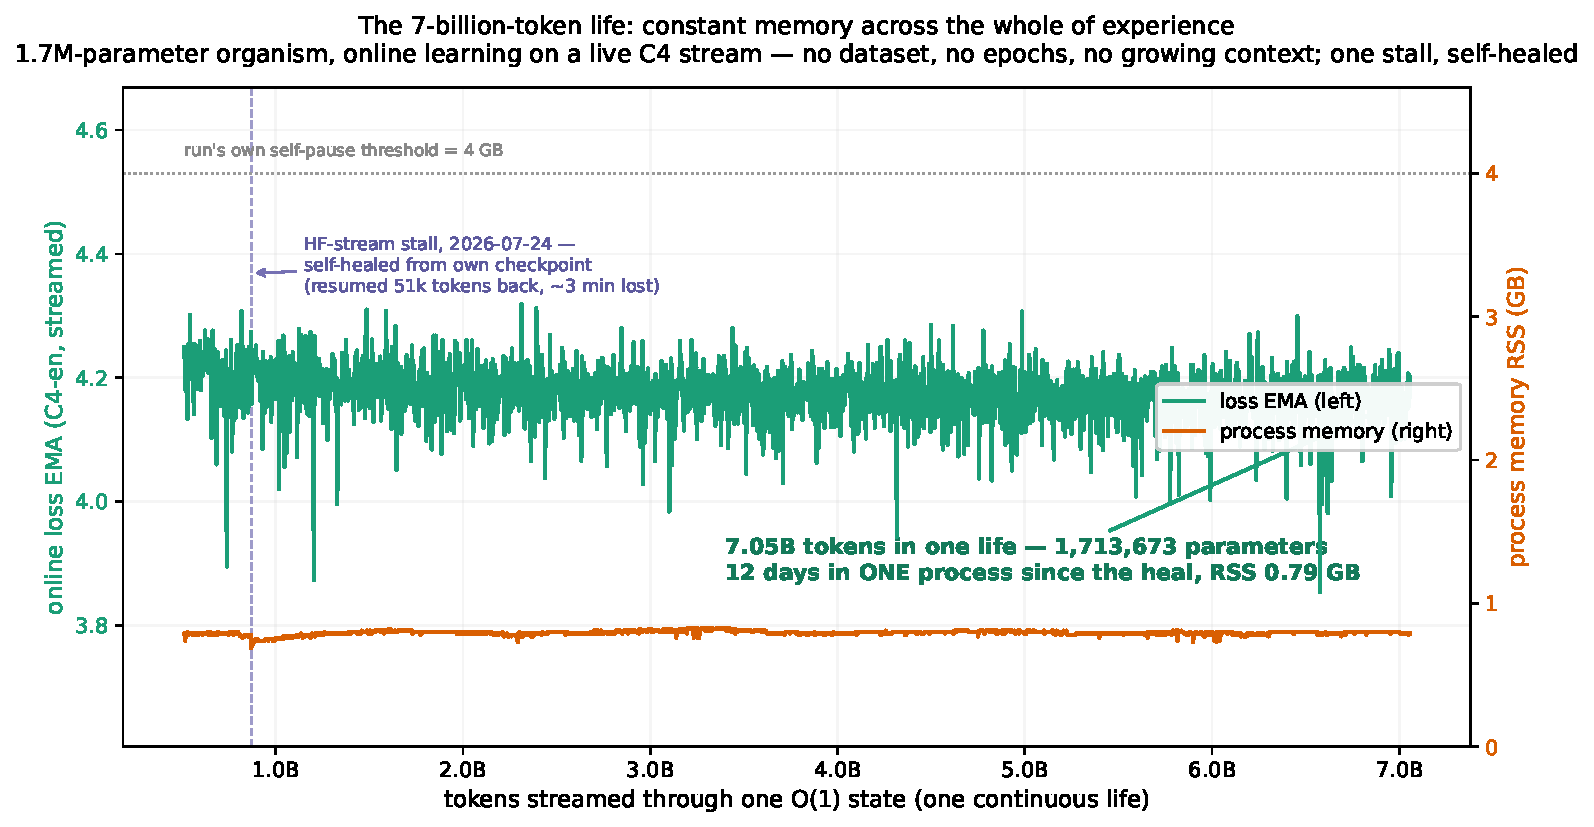
\includegraphics[width=5.20in]{fig_lifetime_7b.pdf}
\caption{Constant memory across a lifetime. Loss EMA (left axis) and process
RSS (right axis) against tokens streamed through one bounded state. Memory
stays inside \num{0.69}--\num{0.83}~GB across nearly four orders of magnitude
of experience; the single interruption self-heals from the run's own atomic
checkpoint. Sources: \code{results/lifetime\_7b\_series.json},
\code{results/lifetime\_7b\_curve.json}.}
\label{fig:lifetime}
\end{figure}

\section{Composition as a stabilizer (brief; see companion)}
\label{sec:composition}

The operating primitives measured above --- surprise-gated plasticity, the
span store, dosed replay under a dividend monitor, reminder injection --- are
not independent knobs; composed into one process they stabilize each other. At
6.7$\times$ the exposure of the original shock protocol, the composed organism
beats the best single-organ regime on all three continual-learning axes ---
forgetting \textbf{$+\num{0.381132}$} against $+\num{1.306251}$, plasticity
$+\num{0.672334}$ against $+\num{0.630965}$, and residual after recovery
$-\num{0.040215}$ (it degrades least, so it has least to recover) --- while
spending \textbf{41\% fewer gradient tokens} (\num{426496} against
\num{718336}; \code{results/chimera\_v1.json}, all four registered clauses
pass). The finding that outranks the table is a stability law: under
6.7$\times$ exposure the single-organ regime degrades near-linearly (forgetting
\num{0.189}$\to$\num{1.306}) while the composition degrades sublinearly
(\num{0.259}$\to$\num{0.381}). For deployment this means the composed system is
not merely cheaper --- it is what keeps the parts working as exposure grows.
The full ablation, with each organ's attributed contribution, is the subject of
the companion paper's composition section.

\section{Related work}
\label{sec:related}

The systems framing here draws on four literatures without belonging wholly to
any of them. \textbf{Continual learning} studies plasticity against forgetting;
we adopt replay as the mechanism \cite{vandeven2019replay} but drive the
selection from the learner's own surprise rather than a curator, and we carry
no weight-space penalty \cite{kirkpatrick2017ewc} in the loop --- the
forgetting control is the frozen external file, not a regularizer on the
weights. \textbf{Model merging} fuses independently trained weights into one
\cite{wortsman2022modelsoups, matena2022merging}; our replication results say
where weight fusion is safe (the companion measures that bounded-divergence
averaging beats its parts while full-divergence one-shot merging loses) and,
more to the present point, that the primary sharing channel between organisms
is not weight space at all but the kilobyte-scale span store.
\textbf{Federated and distributed learning} coordinates many learners over a
network \cite{mcmahan2017fedavg}; the two-regime replication law
(\S\ref{sec:replication}) is the rate-level feasibility condition for keeping
such copies synchronized against a \emph{live} source, which the federated
setting --- synchronizing against a fixed objective --- does not face. And the
\textbf{live migration of virtual machines} \cite{clark2005livemigration} is
the closest systems analogy: a running computation moved between hosts with
bounded disruption. The organism makes the analogy exact --- its complete state
is a small serializable artifact --- and adds what a VM does not have: the moved
state is behaviorally reproducible to the bit, so migration parity is a
measurable identity rather than a best-effort. The operator substrate is the
selective state-space family \cite{gu2023mamba}; the companion paper measures
the family reduction and the exactness license that make streaming training
exact.

\section{Limitations and open problems, as build paths}
\label{sec:limits}

Each measured limit below points at a specific construction; none is a soft
spot in the thesis, and each is stated with the number that bounds it.

\paragraph{Chase needs equal-or-faster hardware.} The two-regime law
(\S\ref{sec:replication}) is exact about when chase replication fails: on an
unequal pairing the source-rate$\times$follower-cost product read \num{2.35} and
the debt diverged \num{10000}$\to$\num{19000} chunks in a cycle. This is not a
defect to remove but a rate condition to satisfy --- provision the follower on
equal-or-faster hardware, or use snapshot-sync, which erased a \num{45000}-chunk
deficit in one transfer. The build path is a scheduler that reads the two rates
and picks the regime.

\paragraph{Keyed recall through the file is unbuilt.} Provenance
(\S\ref{sec:provenance}) is bit-exact replay from coordinates, and the file
transfers as a dose; what it does not yet do is answer a keyed query addressed
into its contents. The construction is a read path that indexes the frozen file
by content, and it sits on top of a provenance layer that already holds 5/5
across text, a mutating pixel world, and a third-party engine.

\paragraph{Cross-replica arbitration is unbuilt.} A reader consumes a shared
file; it does not yet arbitrate between conflicting or adversarial entries from
multiple producers. With provenance already attached to every entry (every span
carries its origin coordinates), arbitration is a policy over trusted
coordinates --- a governance layer to add, not a representation to redesign.

\paragraph{Scale and scope.} $d_\text{model}\le 512$ and C4/WT-2-derived
vocabularies; the width curve measures selection efficiency at a fixed token
budget, not model quality, and the lifetime organism's constancy claim is about
resources, not learning (1.7M parameters, capacity floor). Cross-architecture
parity is measured at equal chunk counts only. Wall-clock throughput is never
claimed --- all axes are token-based, precisely because
Figure~\ref{fig:determinism} shows wall time is the one field that does not
reproduce.

\section{Conclusion}
\label{sec:conclusion}

Deployability is decided by systems properties, and the factoring that makes
the organism a constant-memory streaming learner also makes those properties
measurable and favorable. Reproduction is a bit-level identity on the
deterministic record, holding across an eleven-day gap, a process boundary, and
a stream reconnect --- \num{97657} chunks at deterministic-field difference
exactly \num{0.0}. Provenance is bit-exact replay from stream coordinates,
holding in text, through a world mutation, and through a game engine we did not
write, with the file transferring \num{0.056} of benefit to a stranger on an
unseen route. Migration is a behaviorally exact transfer, and replication obeys
a two-regime law computable in advance from two rates, with the folk
``$2\times$'' cost decomposed to $1.032\times$. And the operating cost ---
memory constant inside \num{0.69}--\num{0.83}~GB across \num{7053926400} tokens,
selection rate deterministic per configuration --- is a quantity you evaluate
before you run. The organism is not only something that learns on a stream; it
is something you can reproduce, move, replicate, and account for --- an asset,
with the systems guarantees an asset needs. Everything here reruns from the
repository.

{\small
\bibliographystyle{plain}
\bibliography{systems_v01_refs}
}

\end{document}
